\chapter{レンダリングプロトコル}

3Dアプリケーションとコンポジッタとの間のプロトコルの中でも特に重要であるのが,
アプリケーションの表示に関するレンダリングプロトコルである.
レンダリングプロトコルに求められるものには以下のものがある.

\begin{itemize}
  \item 複数のアプリケーションが別々に提示してきたレンダリングの情報を合成して,
        1つの没入環境に矛盾なくレンダリングできる.
  \item 質の悪いアプリケーションが他のアプリケーションや環境全体に影響を及ぼさない.
        複数のアプリケーションを利用できる環境下では,質の悪いアプリケーションがあり,
        フレームレートにレンダリングが追いつかなかったり,ハングしてしまう可能性がある.
        このようなときにシステム全体への影響を最小限にする必要がある.
  \item レンダリングの効率がよい.
  \item レンダリングの自由度が高く,様々な表現が可能である.
        % \item Motion-to-photon(MTP) latency(ユーザが動いてから,その動きを反映させて
        %       レンダリングした結果の映像が目に届くまでの時間)を小さくできる.
        %       MTP latencyが大きくなるとVRやARにおけるPresenceの低下や
        %       motion sicknessを引き起こすと言われている.
        % 軽減手法を入れてもいいかも
\end{itemize}

\section{3Dコンピュータグラフィックス}
\label{section:3DCG}

この節では以降の説明のために最小限必要な,3Dレンダリングにおけるレンダリングパイプラインの
概要を述べる.
ただしレンダリングの手法は様々であり,ここでは代表的な手法についてのみ述べている.

3Dオブジェクトのレンダリングは基本的に,3D空間で定義されたオブジェクトを,ある視点から見た
時の2次元平面でのピクセルマップに落とし込む行為である.
このプロセスは大きく,Geometry ProcessingとRasterizationの2つのフェーズに
分けることができる.

\subsection*{Geometry Processing}

3Dオブジェクトの形は多くの場合,メッシュによって表現され.メッシュは三角形などのPrimitiveの
集まりとして表現される.
レンダリングパイプラインではこのPrimitiveごとに,それがScreenのどのピクセルを何色で
塗りつぶすかを計算する.
Geometry Processingのフェーズ(図\ref{fig:geometry-processing})
ではこのPrimitiveを構成する頂点の座標(Object Space)を行列計算によって,
ある視点から投影したときの座標(Clip Space)へ変換するフェーズである.
Primitiveの頂点はまず,Model Matrixをかけることで,World Spaceのどこに配置するかが決定される.
さらにこれに,視点の位置や向き,視野角などから取得されるView Projection Matrixを乗算することで,
頂点はClip Spaceに配置される.

これらの操作はVertex Shaderによって制御される.OpenGL
\footnote{Khronos Group "OpenGL" https://www.opengl.org/ (accessed 27 Dec, 2022)}
のシェーダ言語であるGLSLにおける簡単なVertex Shaderの例を
ソースコード\ref{code:vertex-shader}に示した.
ここでのmodel,view\_projectionはUniform変数などと呼ばれ,その値は
レンダリングパイプラインを実行するときに指定できる.

\begin{figure}[htbp]
  \centering
  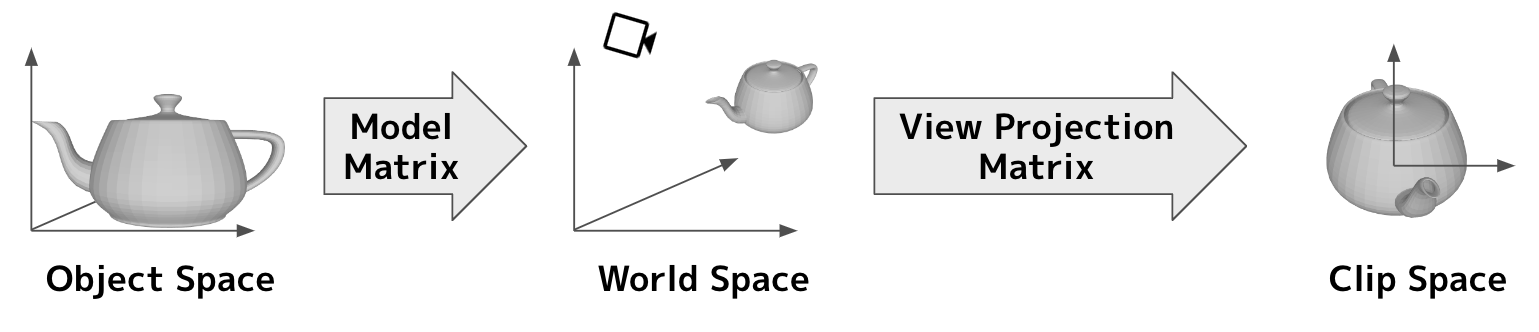
\includegraphics[keepaspectratio, width=\linewidth]{figures/geometry-processing.png}
  \caption{
    Geometry Processing.
  }
  \label{fig:geometry-processing}
\end{figure}

\begin{lstlisting}[caption=Vertex Shaderの例, label=code:vertex-shader]
uniform mat4 model;
uniform mat4 view_projection;
layout(location = 0) in vec4 position;

void main() {
  gl_Position = view_projection * model * position;
}
\end{lstlisting}

\subsection*{Rasterization}

Clip Spaceに変換されたPrimitiveはRasterizationのプロセスによって,
スクリーン上のどのピクセルをどの色で塗るかといった情報にまで落とし込む.
このピクセルごとの情報はフラグメントと呼ばれ,一般的にフラグメントには色の情報と,
そのフラグメントに投影されたPrimitiveが視点からどれくらい離れているかを指す深度情報が含まれる.
このRasterizationのフェーズではFragment Shaderやテクスチャなどをプログラマが指定する.

\subsection*{Framebuffer と Depth Testing}

Framebufferとはレンダリング結果を格納するバッファである.
Framebufferはピクセルごとの色の情報を保持するColor bufferと
深度の情報を保持するDepth bufferを含むことが多く,Rasterizationによって得られた
フラグメントはFramebufferのColor bufferとDepth bufferに格納される.
RasterizationによってPrimitiveがフラグメントに変換され,そのフラグメントが次々と
Framebufferに書きこまれていくが,このときDepth Testingを用いると,
フラグメントの深度情報とFramebufferが持つ深度情報とを比較して,
フラグメントが手前にあるときだけ,Framebufferに書き込むということができる.
これによって,重なっているPrimitiveの処理順に関係なく,Primitiveの前後関係を
レンダリングに反映させている.

\subsection*{レンダリングパイプライン}

今まで述べたプロセスはレンダリンパイプラインとして,GPU内で行われることが多い.
ただしレンダリングパイプラインを実行するために必要なデータはプログラマによって
CPUで作成され,OpenGLなどのAPIを通してGPUに送られるのが一般的である.
レンダリングパイプラインへの入力としては主に以下のものがある.

\begin{itemize}
  \item メッシュに関するデータ:頂点の位置情報やそれに付随するデータなど.
  \item テクスチャ
  \item Model Matrix の値
  \item View Projection Matrix の値
  \item Vertex / Fragment Shader
\end{itemize}

\section{関連技術・研究}

本システムはそれぞれ別プロセスのアプリケーションがレンダリングしたい情報を持っており,結果的に
1つのレンダリング結果を導くという点でParallel Renderingの分野と類似性がある.
MolnarらはParallel Renderingの手法を``sort-first'', ``sort-middle'', ``sort-last''の
大きく3つに大別した\cite{parallel-rendering}(図\ref{fig:parallel-rendering}).
\ref{section:3DCG}で述べたとおり,3DレンダリングはPrimitiveがどのピクセルに影響を与えるかを
計算するタスクであり,Primitiveをスクリーンへとsort(選別・分配)するタスクであると捉えられる.
Parallel Renderingにおいてこのsortのタスクでは,プロセッサ間でPrimitiveやフラグメントに
関するデータを再配置する必要がある.
Molnarらはこの再配置のタイミングに注目しており,``sort-first''は,Primitiveを
Geometry Processingの際に再配置する手法,``sort-middle''はGeometry Processing後の
Primitiveを再配置する手法,そして``sort-last''はRasterizationの際にフラグメントなどを
再配置する手法である.

\begin{figure}[htbp]
  \begin{minipage}[t]{0.32\linewidth}
    \centering
    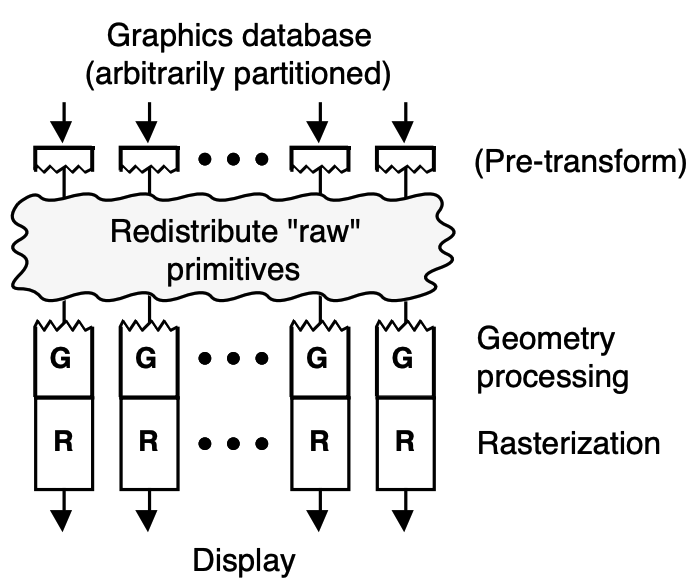
\includegraphics[keepaspectratio, width=\linewidth]{figures/sort-first.png}
    \subcaption*{Sort-first}
  \end{minipage}
  \begin{minipage}[t]{0.32\linewidth}
    \centering
    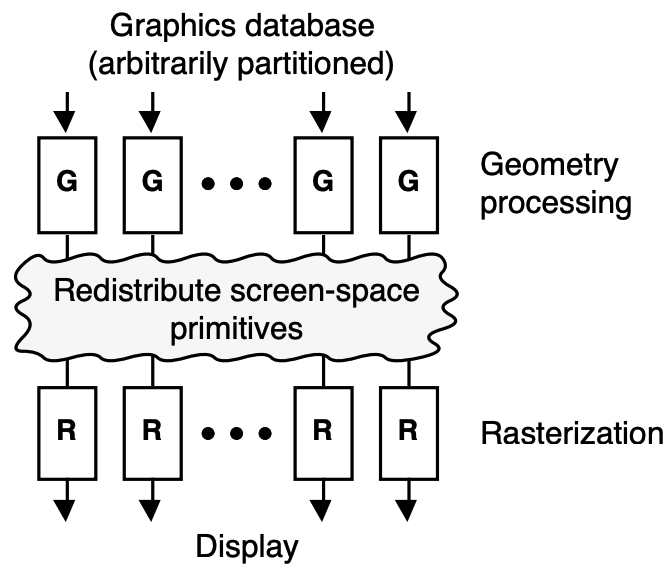
\includegraphics[keepaspectratio, width=\linewidth]{figures/sort-middle.png}
    \subcaption*{Sort-middle}
  \end{minipage}
  \begin{minipage}[t]{0.32\linewidth}
    \centering
    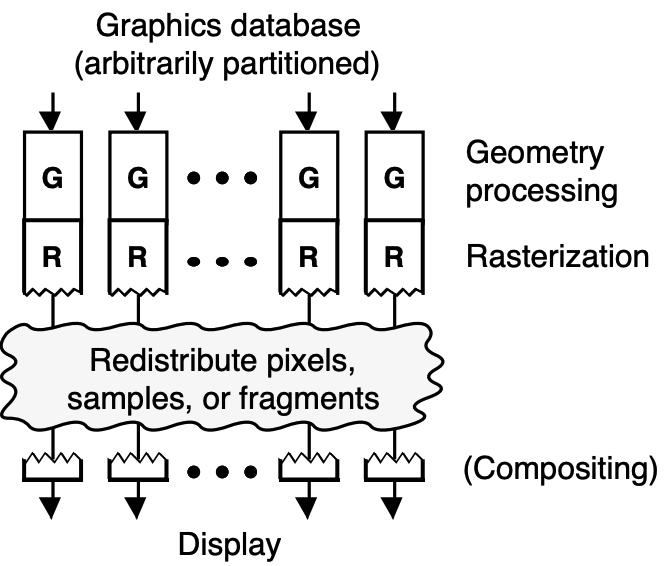
\includegraphics[keepaspectratio, width=\linewidth]{figures/sort-last.png}
    \subcaption*{Sort-last}
  \end{minipage}
  \caption{
    Molnarらによって分類されたParallel Renderingの3つの手法.
    (Each figure is adapted from Molnar, at el. 1994\cite{parallel-rendering})
  }
  \label{fig:parallel-rendering}
\end{figure}

本研究では,複数のアプリケーションがコンポジッタに対してレンダリングに必要な情報を伝達して,
それを用いてコンポジッタ側が最終的なレンダリングを行うため,Molnarらの分類において,
データの分配のタイミングまでをアプリケーションが担い,分配後をコンポジッタが担うと捉えられる.
ただしMolnarらの設定とは大きな違いがあり,Molnarらの論文ではスクリーンはいくつかの領域に
分割され,その領域ごとにプロセッサが割り当てられてレンダリングを行う設定であったため,
どのプロセッサにデータを再配置するかを知るために,データがスクリーンのどの領域に
影響を与えるものであるか計算できている必要があった.
一方本研究の設定では,アプリケーションがデータを作成しコンポジッタで合成するために
データの再配置(アプリケーションからコンポジッタへの描画情報の伝達)をおこなう.
全く異なる設定ではあるが,Molnarらの論文での洞察や検証は本研究にも応用できる部分が多い.

Reilingの提案したmotorcar\cite{reiling}は
``sort-last''に近い手法(図\ref{fig:reiling-rendering})をとっている.
motorcarではそれぞれのアプリケーション(図\ref{fig:reiling-rendering}ではclient)が
レンダリングを行い,生成したフレームバッファをできるだけ効率のよい方法でコンポジッタに送り,
Depth Testingによってそれぞれのアプリケーションのフレームバッファどうしを合成している.
motorcarの手法の特徴は以下のとおりである.

\subsubsection*{矛盾のないレンダリングについて}

Depth Testingによって,複数のアプリケーションを矛盾なく合成できる.

\subsubsection*{質の悪いアプリケーションについて}

質の悪いアプリケーションがフリーズしてしまった場合などは,オブジェクトが消えてしまうか,
視点の情報を更新できず,描画の整合性が失われてしまう.

\subsubsection*{レンダリングの効率について}

複数のアプリケーションがGPUを共有するため,プロセス間でGPUを奪い合い,
コンテキストスイッチにオーバヘッドがある.
また,Molnarらが指摘しているとおり,``sort-last''の手法ではコンポジッタに対して毎フレーム
全てのフラグメントの情報を送る必要があり,データの転送量が多くなってしまう.
Reilingの手法では単一ホストマシン内でのデータ転送であるため,アプリケーションとコンポジッタで
共有したバッファを用いることで時間がかかるGPUメモリへの読み書きを最小限に抑え,
伝達効率を上げているが,Reiling自身が言及されているとおり,
バッファへの書き込みや読み出しの部分でオーバヘッドが存在する.

\subsubsection*{レンダリングの自由度について}

アプリケーションがレンダリングパイプラインを全て実行できるため,描画の自由度が高い.
ただし,他のアプリケーションのオブジェクトの形などの情報は取得できないため,
他のアプリケーションの影を落とすといったことはできない.

% \subsubsection*{MTP latencyについて}

% motorcarではHMDなどのデバイスから取得される視点の情報がアプリケーションに伝えられ,
% アプリケーションでレンダリングを行って結果がコンポジッタに戻ってくる.
% このため,コンポジッタ側では最低でも次のフレームタイミングよりも,
% アプリケーションで行われるレンダリングの時間分だけ早くその視点の情報を伝える必要がある.
% しかしこの時間を短く見積もってしまうと,アプリケーションのレンダリングが間に合わず,
% フレーム落ちを発生させてしまう.

\begin{figure}[htbp]
  \centering
  \fbox{
    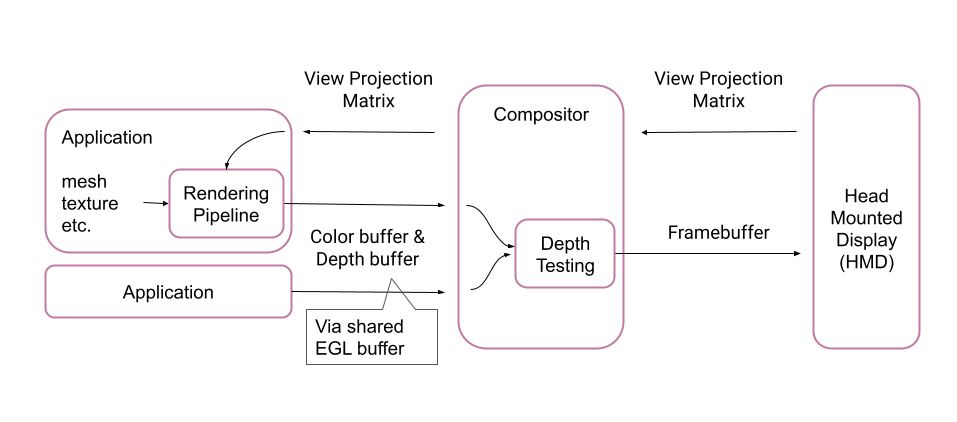
\includegraphics[keepaspectratio, width=0.9\linewidth]{figures/reiling-rendering.png}
  }
  \caption{
    motorcar\cite{reiling}でのレンダリング手法の概略図.
  }
  \label{fig:reiling-rendering}
\end{figure}

Peuhkurinenらはmotorcarの手法におけるコンテキストスイッチのオーバヘッドを指摘し,
アプリケーションとコンポジッタとの間で共有したシーングラフを用いる手法を提案した\cite{peuhkurinen}.
Peuhkurinenらはモバイル端末を用いたAR環境で実験をしているため,没入環境ではないが,
端末の位置や傾きをもとに,複数のアプリケーションをAR環境にレンダリングしている点で,
レンダリングに関しては本研究と同じ問題に取り組んでいる.
Peuhkurinenらの手法(図\ref{fig:peuhkurinen-rendering})ではコンポジッタ側で
1つのシーングラフを持ち,アプリケーションがIPCによってそのシーングラフに変更を加える.
コンポジッタでは毎フレームそのシーングラフを走査し,そのタイミングで取得した
デバイスの位置や傾きを使ってシーンをレンダリングする.
Peuhkurinenらの手法の特徴は以下のとおりである.

\subsubsection*{矛盾のないレンダリングについて}

システムで共有するシーングラフからレンダリングすることで
複数のアプリケーションを矛盾なくレンダリングできる.

\subsubsection*{質の悪いアプリケーションについて}

質の悪いアプリケーションがフリーズした場合でも,シーングラフの更新が途絶えるだけで,
フレームごとにデバイスの位置や傾きを更新して,矛盾なくシーンをレンダリングできる.

\subsubsection*{レンダリングの効率について}

レンダリングは全てコンポジッタ側で行われるため,
コンテキストスイッチのオーバヘッドがなく効率的である.

\subsubsection*{レンダリングの自由度について}

シーングラフの設計によってレンダリングできるものが限られてしまい,レンダリングの自由度は
著しく落ちる.
特にPeuhkurinenらが提案したシーングラフを構成する要素は以下の5つであり,
より高度なレンダリングを実現する提案までは至らなかった.

\begin{enumerate}
  \item \textbf{Mesh}
        位置を表す(X,Y,Z)と頂点の法線ベクトルの(X,Y,Z),UVマッピングのための(U,V)の情報を持つ.
  \item \textbf{Texture}
        8bitずつのRGBAコンポーネントを持つ.
  \item \textbf{Transformation Matrix}
        アプリケーションのローカル座標系におけるMeshの平行移動,回転,スケールを表す4x4の変換行列.
  \item \textbf{Node}
        Mesh,Texture,Transformation Matrixから構成され,コンポジッタによって描画される単位.
  \item \textbf{Application Volume}
        アプリケーションがNodeを描画できる直方体領域.
\end{enumerate}

\begin{figure}[htbp]
  \centering
  \fbox{
    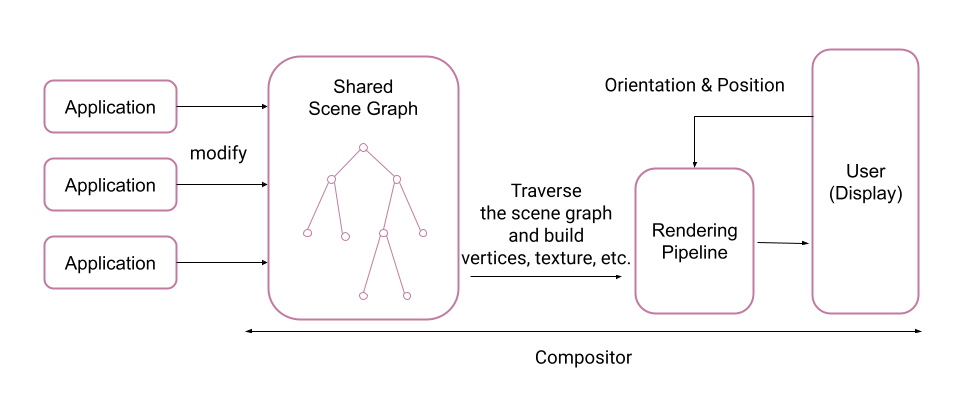
\includegraphics[keepaspectratio, width=0.9\linewidth]{figures/peuhkurinen-rendering.png}
  }
  \caption{
    Peuhkurinenら\cite{peuhkurinen}の提案するシステムのレンダリング手法の概略図.
  }
  \label{fig:peuhkurinen-rendering}
\end{figure}

% sort-first か sort-last かみたいな有名な論文から
% http://www.cs.cmu.edu/afs/cs/academic/class/15869-f11/www/readings/molnar94_sorting.pdf?fbclid=IwAR1oupZA71Gn8IAoOu0F5fJ-GbjJjJH6moYND0nTmtw0w81hqK1qpen7TR4
% Forrestなど、似たことをしようとしているものも

\section{提案手法}

motorcarの手法では,レンダリングの自由度は高いが,レンダリングの効率や
質の悪いアプリケーションがいた場合において問題があった.
一方共有シーングラフを用いたPeuhkurinenらの手法では,レンダリング効率や,
質の悪いアプリケーションに関しては有効だが,レンダリングの自由度が制限されていた.
本システムでは``sort-first''に近い手法を提案し,レンダリングの効率や質の悪いアプリケーションの問題を
解決しつつ,Peuhkurinenらの手法よりレンダリングの自由度を高くする.

本システムでのレンダリング手法の基本的な方針は,シーングラフといった抽象化を行うと
その分レンダリングの自由度が落ちてしまうため,できるだけアプリケーションが
レンダリングパイプラインをそのまま使うことができるようにすることである.
そこで本システムでは広く使われているグラフィックスライブラリであるOpenGLをベースとした
レンダリングプロトコルを作成した.今回は特にOpenGL ES 3.2
\footnote{Khronos Group "OpenGL ES Version 3.2" \url{https://registry.khronos.org/OpenGL/specs/es/3.2/es_spec_3.2.pdf} (accessed 29, Dec)}
をもとにしている.

OpenGLでは以下のようなオブジェクトが定義されており(一部).
これらのオブジェクトといくつかのパラメータを指定してレンダリングパイプラインを実行することで,
指定したFramebufferにレンダリング結果が格納される.
\begin{itemize}
  \item \textbf{Buffer Object} 頂点データや頂点の配列順のデータなどを格納する汎用的なバッファ
  \item \textbf{Shader Objects} Vertex ShaderやFragment Shaderなどを格納するオブジェクト
  \item \textbf{Program Objects} レンダリングパイプラインの各ステージで用いられるShader Objectをひとまとまりにするオブジェクト
  \item \textbf{Texture Objects} テクスチャを格納するオブジェクト
  \item \textbf{Sampler Objects} テクスチャのサンプリングに関するパラメータの集合を保持するオブジェクト
  \item \textbf{Vertex Array Objects}
        Vertex Shaderで用いる頂点情報がどのバッファのどこに,どのような形式で存在するかを指定するオブジェクト
        % \item \textbf{Framebuffer Objects} Framebufferとその状態を保持するオブジェクト
\end{itemize}

本システム(図 \ref{fig:rendering})ではまず,アプリケーションがIPCを用いて上記の6つの
オブジェクト(Rendering Resource)をコンポジッタ側で作成するプロトコルを用意した.
また,レンダリングパイプライン実行時に指定するオブジェクトとパラメータをまとめた
Rendering Unitというオブジェクトを新たに定義した.Rendering Unitは
1回のレンダリングパイプラインの実行に相当する.
そして,アプリケーションがRendering Unitをコンポジッタ側に作成し,
Rendering Unitに対してRendering Resourceの紐付けと,パラメータの指定をできるようにした.
Rendering Resourceは複数のRendering Unitに対して紐づけることが可能である.
また,Rendering Unitに対して指定可能なパラメータには,
シェーダから利用可能なUniform変数の値などを含む.

\begin{figure}[htbp]
  \centering
  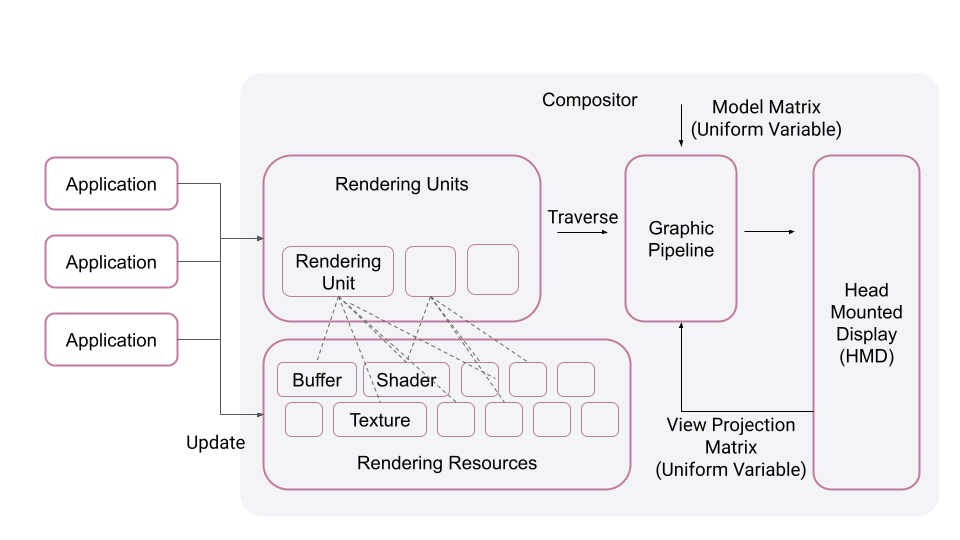
\includegraphics[keepaspectratio, width=1\linewidth]{figures/rendering.png}
  \caption{
    本システムのレンダリング手法の概要図.
  }
  \label{fig:rendering}
\end{figure}

上記のようなシステムにすることで,アプリケーションは頂点データの形式,バッファへの格納方法,
テクスチャの形式,そしてシェーダを自由に設定,記述でき,
レンダリングの自由度を高く保つことができた.
また,レンダリングパイプラインの実行自体は全てコンポジッタ側で行われるため,
GPUのコンテキストスイッチが少なく,効率的である.
TextureやBuffer,Shaderなどのサイズの大きいオブジェクトはその生成やフォーマットの修正,
転送のコストも無視できないが,本システムではアプリケーションは共有メモリを介してそれらの
オブジェクトをコンポジッタと共有し,コンポジッタはそのデータを再形成することなくそのまま
GPU上のメモリに転送できるため,転送や再形成のためにオーバヘッドがかかることはない.
最後に,質の悪いアプリケーションに対応するための工夫を述べる.

\ref{section:overview:windowing-system}で述べたとおり,
マルチコンテキストな没入環境を実現するためには,アプリケーション間の衝突を防ぎ,
適切に分離することが大切である.
そのため質の悪いアプリケーションがフリーズしたり,動作が遅くなった場合でも,
そのアプリケーションをレンダリングする際の視点情報が更新される必要がある.
そうでなければ,アプリケーションのレンダリング情報が途絶えた場合に,
そのアプリケーションのレンダリングをやめるか,最後のレンダリング結果を表示し続けることになる.
前者の場合はチラつきが発生し,後者の場合は現在の視点と異なる視点でレンダリングした結果を
表示するため,整合性が失われ,酔いの原因になりうる.
いずれにせよ,1つのアプリケーションが環境全体にあたえる影響が大きい.
視点情報が更新され続ければ,フリーズしたアプリケーションがレンダリングするオブジェクトは
没入環境の中では静止するが,描画の整合性が失われることはなく,
他のアプリケーションは通常通り利用できる.

また,本システムではアプリケーションの位置をコンポジッタ側が決定する.
これはユーザがアプリケーションを好きな位置に配置し,アプリケーションどうしの空間的な衝突を
ユーザが最小限にできることを保証するためであるが,フリーズしたり,動作が遅いアプリケーションでも
その配置を変更できるようにする必要がある.
そのため質の悪いアプリケーションがフリーズしたり,動作が遅くなった場合でも,アプリケーションの
配置を決めるModel Matrixが更新可能である必要がある.

以上の議論から,レンダリングする際にModel Matrixと視点の情報である
View Projection Matrixをいかに適用するかが重要である.
\ref{section:3DCG}で述べたように,通常Model MatrixやView Projection Matrix は
Uniform変数として用い,シェーダで頂点に対して適用することが多い.
一般的な既存のVRアプリケーション(図\ref{fig:app-mvp})では
ソースコード\ref{code:vertex-shader}のようなVertex Shaderと,そのVertex Shaderで
用いられているModel MatrixやView Projection Matrixを示すUniform変数に入れる値を
Graphics Pipelineに伝えることで,頂点にModel MatrixとView Projection matrix
を適用させている.

\begin{figure}[htbp]
  \centering
  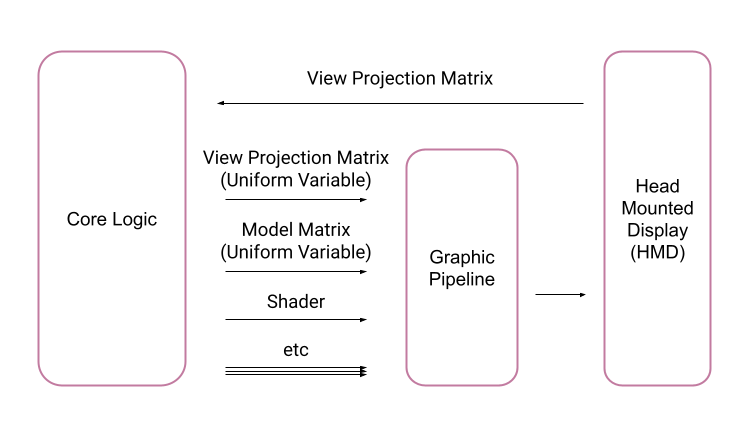
\includegraphics[keepaspectratio, width=1\linewidth]{figures/app-mvp.png}
  \caption{
    没入環境での一般的なアプリケーションでのMode View Projection Matrixの適応のさせ方の例.
  }
  \label{fig:app-mvp}
\end{figure}

本システムのレンダリングシステムでは(図\ref{fig:rendering}),Model Matrixは
コンポジッタがアプリケーションごとに管理しているものを,View Projection Matrixは
HMDから取得したものをアプリケーションへ渡すことなくGraphics Pipeline実行時に適用する.
そのため本システムではシェーダで用いるUniform変数のいくつかを予約しており,
例えば``zModel''という名前のUniform変数にはModel Matrixの値を,
``zViewProjection''というUniform変数にはView Projection Matrixの値をコンポジッタ側で
設定することとしている.
アプリケーションはソースコード\ref{code:zigen-vertex-shader}のようなVertex Shaderを
記述することで,Model MatrixやView Projection Matrixの実際の値を知らないまま,
用いることができる.

\begin{lstlisting}[caption=本システムでのVertex Shaderの例, label=code:zigen-vertex-shader]
  uniform mat4 zModel;
  uniform mat4 zViewProjection;
  layout(location = 0) in vec4 position;
  
  void main() {
    gl_Position = zViewProjection * zModel * position;
  }
\end{lstlisting}

このように本システムでは,Model MatrixとView Projection Matrixを表すUniform変数の値を
コンポジッタ側が,それ以外のレンダリングパイプラインの実行に必要なオブジェクトやパラメータを
アプリケーション側が提供し,コンポジッタ側でレンダリングパイプラインを実行する.
これにより,レンダリングに関するオーバヘッドが小さく,レンダリングの自由度を高く保ち,
かつ質の悪いアプリケーションに対して堅牢なレンダリングシステムを実現した.
% アプリケーションの質が悪く,フリーズしたり,動作が遅い場合に本システムでは
% アプリケーションがフリーズした場合や動作が遅い場合でも,視点の移動をレンダリングに反映させ
% 続けるためには,視点情報をアプリケーションに送らないことが重要である.
% Peuhkurinenらの手法でも視点情報はコンポジッタ側で保持していた.

% 視点情報を送らない

\section{評価:レンダリング性能}

本節では,レンダリング性能に関して絶対的な評価をした.

\subsection{実装・環境}

プログラミング言語はCとC++を用いた.
アプリケーションとコンポジッタ間のIPCにはWaylandを用いた.
HMDへの出力,HMDからのView Projection Matrixの取得にはSteamVRランタイムのOpenVRを用いた.
その他の環境に関しては表\ref{table:rendering-env}に示す.

\begin{table}[htbp]
  \centering
  \begin{tabular}{|r||l|}
    \hline
    OS     & Ubuntu 20.04.4 LTS                        \\
    \hline
    Kernel & 5.13.0-41-generic                         \\
    \hline
    CPU    & Intel(R) Core(TM) i7-10700K CPU @ 3.80GHz \\
    \hline
    GPU    & GeForce RTX 2070 SUPER                    \\
    \hline
    Memory & 32GB                                      \\
    \hline
    HMD    & Valve Index                               \\
    \hline
  \end{tabular}
  \caption{レンダリングに関する実験環境}
  \label{table:rendering-env}
\end{table}

また,今回の実装ではFPSの上限は90fpsとなっている.

\subsection{実験の設定}

本実験ではレンダリングの性能を確かめるため,いくつかのタイプの3Dアプリケーションを複数実行し,
システム全体のFPSの変化を測定した.
実験に用いたアプリケーションは以下の3つである.

\subsubsection*{Box App}

Box App(図\ref{fig:box-app})は立方体を表示する,頂点の少ない簡単なアプリケーションである.
ただし一面にテクスチャが貼られており,アプリケーションは毎フレームテクチャを更新する.
テクスチャのサイズは256x256で1ピクセルあたりビット数は32bitである.

\begin{figure}[htbp]
  \centering
  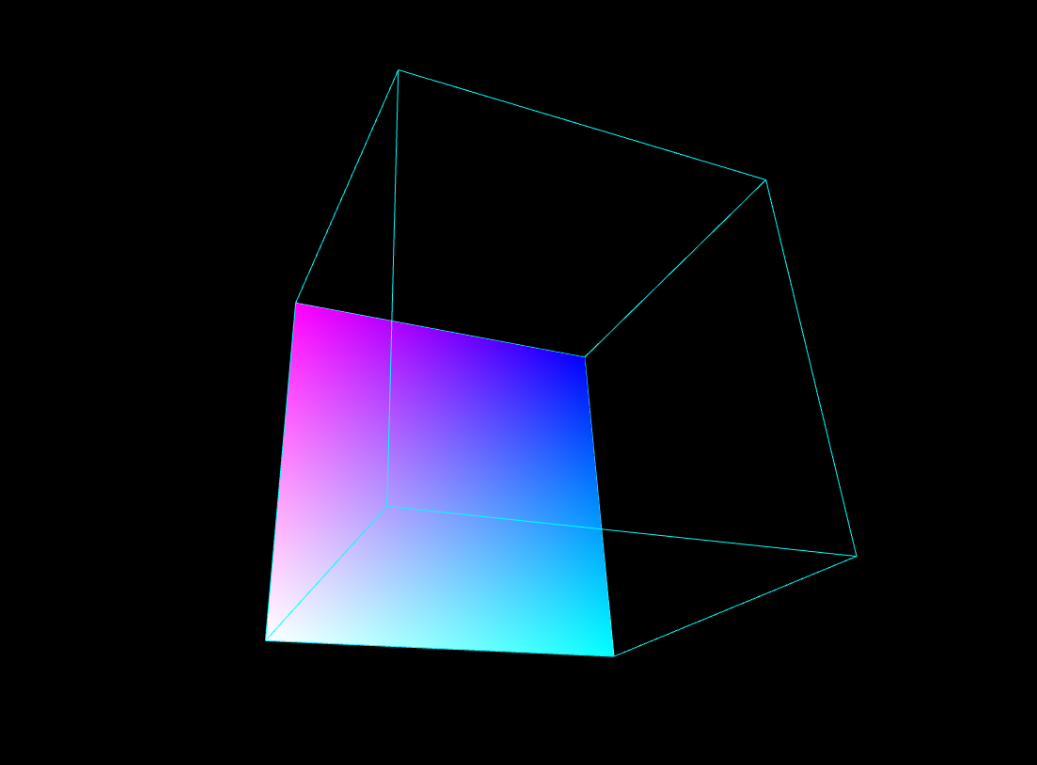
\includegraphics[keepaspectratio, width=0.6\linewidth]{figures/box-app.png}
  \caption{
    Box App.頂点が少なく,テクスチャの更新がある.
  }
  \label{fig:box-app}
\end{figure}

\subsubsection*{STL App}

STL App(図\ref{fig:stl-app})は
STL\footnote{Wikipedia. ``STL(file format)'' \url{https://en.wikipedia.org/wiki/STL_(file_format)} (accessed 17 Jan, 2023)}
形式のファイルを表示するアプリケーションである.
比較的頂点数が多いが,データの更新がない.
本実験で用いたSTLファイルは頂点数が324,000個のものである.

\begin{figure}[htbp]
  \centering
  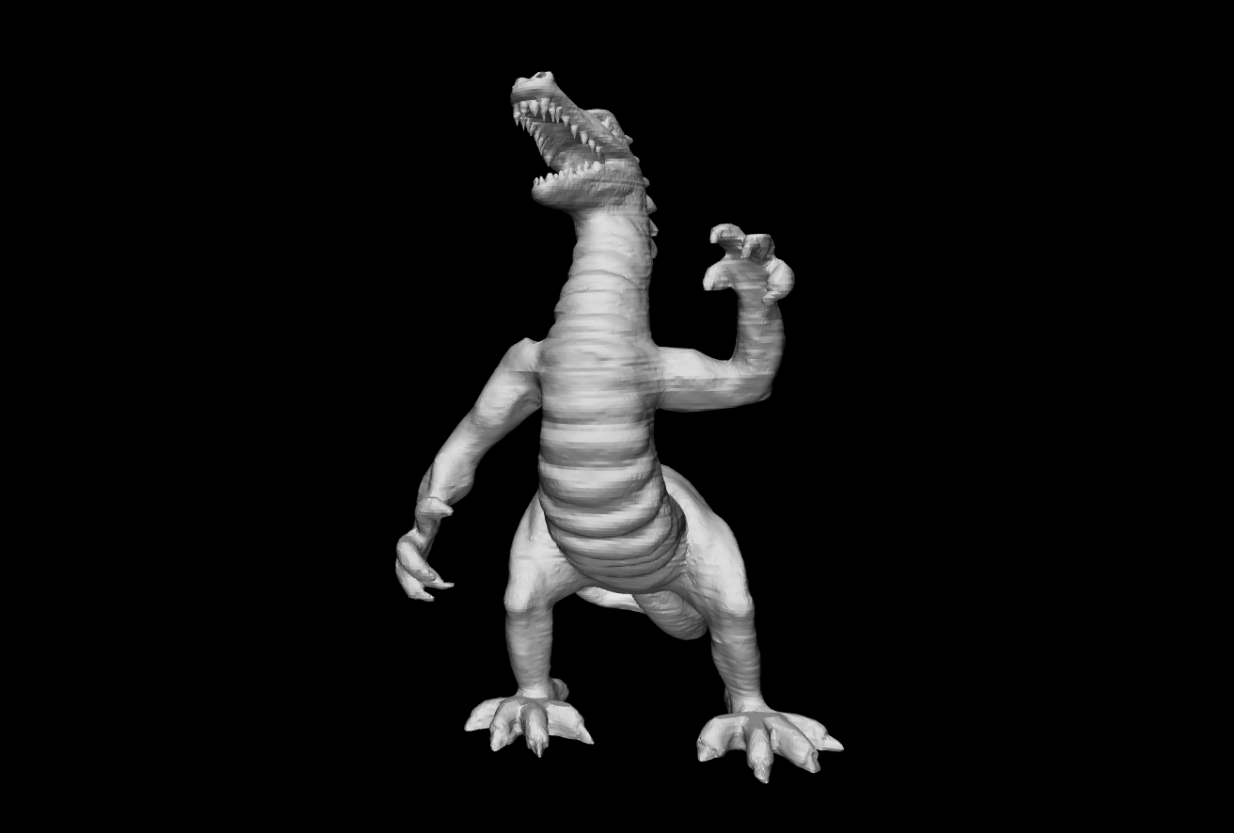
\includegraphics[keepaspectratio, width=0.6\linewidth]{figures/dragon-app.png}
  \caption{
    STL App.頂点が多いが,データの更新がない.
  }
  \label{fig:stl-app}
\end{figure}

\subsubsection*{STL App with rotation}

STL App with rotationはSTL Appに加え,STL オブジェクトをヨー方向に回転させる.
アプリケーションは回転量を表すUniform変数(float, 32bit)を毎フレーム更新し,
頂点シェーダで頂点の回転処理を記述している.

\subsection{結果}

上記の三種類のアプリケーションそれぞれについて,同時に起動するアプリケーションの数を
増やしたときのFPSの変化を図\ref{fig:rendering-fps}に示す.

\begin{figure}[htbp]
  \centering
  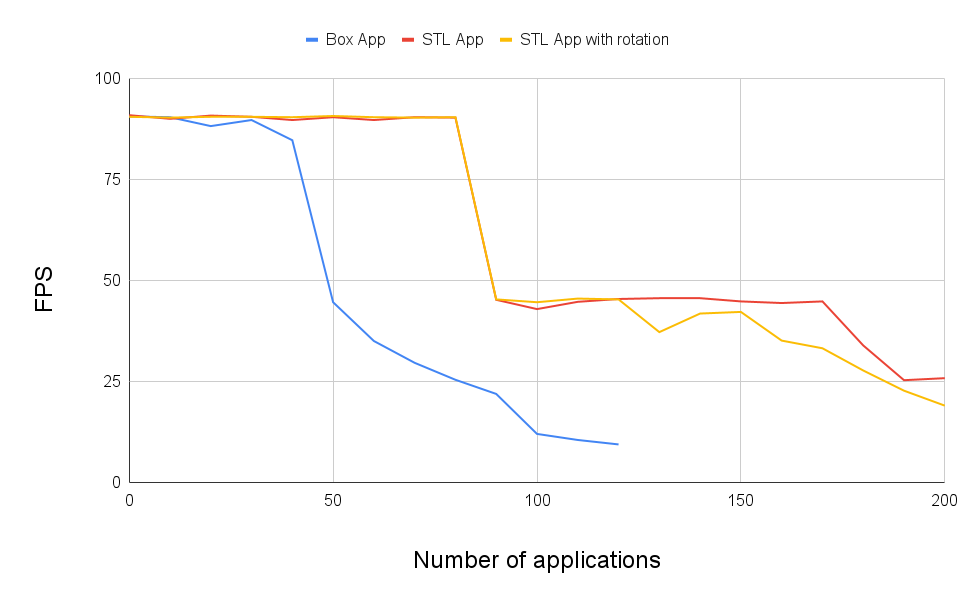
\includegraphics[keepaspectratio, width=\linewidth]{figures/rendering-fps.png}
  \caption{
    レンダリング性能測定実験の結果.
  }
  \label{fig:rendering-fps}
\end{figure}

いずれのタイプのアプリケーションでも40個ほどまでは90fps近くを保っており,
本レンダリング手法が十分実用に耐えうることが示された.
また,STL App や STL App with rotationのように,頂点データ数が多くても
時間あたりに更新するデータが少ないアプリケーションであれば,さらに多くのアプリケーションを
レンダリングできることがわかった.

STL AppとSTL App with rotationにおいて,アプリケーション数が90個近くなったときに
急激にFPSが落ち込むのは,頂点数が多く,レンダリングパイプラインの処理が1フレーム内に
収まりきらなくなり,バッファのスワップが次のフレームタイミングで行われるようになったためである.
一方Box Appでは比較的連続的にFPSが落ちるが,これはコンポジッタ側でアプリケーションから
共有されたテクスチャをGPUへ送る部分に時間がかかっており,コンポジッタのメインループが
ビジー状態になっていることが原因である.

\section{評価:レンダリングの自由度}

この章では様々なレンダリング手法が本レンダリングシステムで適応できることを示し,
レンダリングの自由度が高いことを示す.

\subsection{フラグメントシェーダでのRay Marchingを用いたメタボール}

Ray Marchingはメッシュを用いずにRayを走査することでレンダリングを行う技法の1つであり,
数学的な幾何構造の可視化\cite{ray-marching-math}に用いられたり,
より高度なレンダリング手法\cite{ray-marching-advanced1}\cite{ray-marching-advanced2}
の基礎として用いられる.

メタボール\cite{meta-ball}とはメタボールどうしが近づくことで,
一定の規則に沿ってそれらのメタボールが融合し,ひとかたまりとなる球状のオブジェクトである.

ここではフラグメントシェーダ内でのRay Marchingの一種である
Sphere Tracing\cite{sphere-tracing}を実装し,本システムで
メタボールを表現可能であることを確認した(図\ref{fig:meta-ball}).

\begin{figure}[htbp]
  \centering
  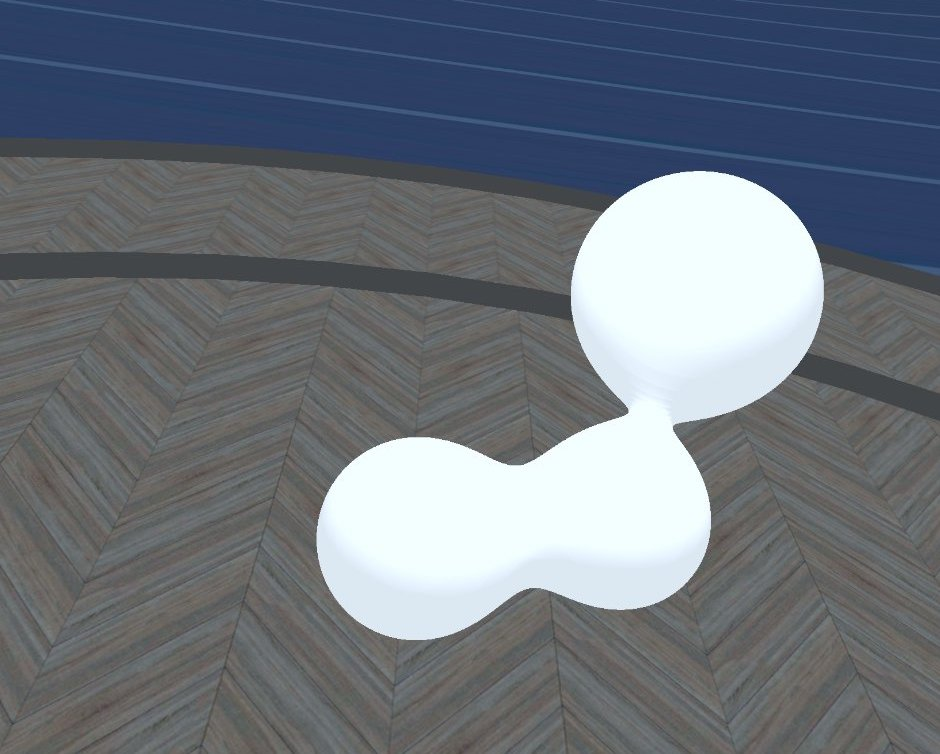
\includegraphics[keepaspectratio, width=0.7\linewidth]{figures/meta-ball.png}
  \caption{
    本レンダリングシステムでSphere Tracingを用いてメタボールをレンダリングする様子.
  }
  \label{fig:meta-ball}
\end{figure}

\subsection{Geometry Shaderを用いた頂点の追加と変換}

\ref{section:3DCG}では主なシェーダとしてVertex ShaderとFragment Shaderを説明したが,
OpenGLではその他にもGeometry ShaderやTesselation Shaderなどがあり,
これらはレンダリングの効率化\cite{geometry-shader-research1}や,
より高度な表現\cite{geometry-shader-research2}のために用いられることがある.


本システムではOpenGLのAPIを踏襲しているため,これらのシェーダを利用してレンダリングを
行うこともできる.
ここでは本レンダリングシステムでGeometry Shaderを用いて,メッシュにポリゴンを追加したり,
頂点を編集したりできることを確かめた(図\ref{fig:geometry-shader}).

\begin{figure}[htbp]
  \centering
  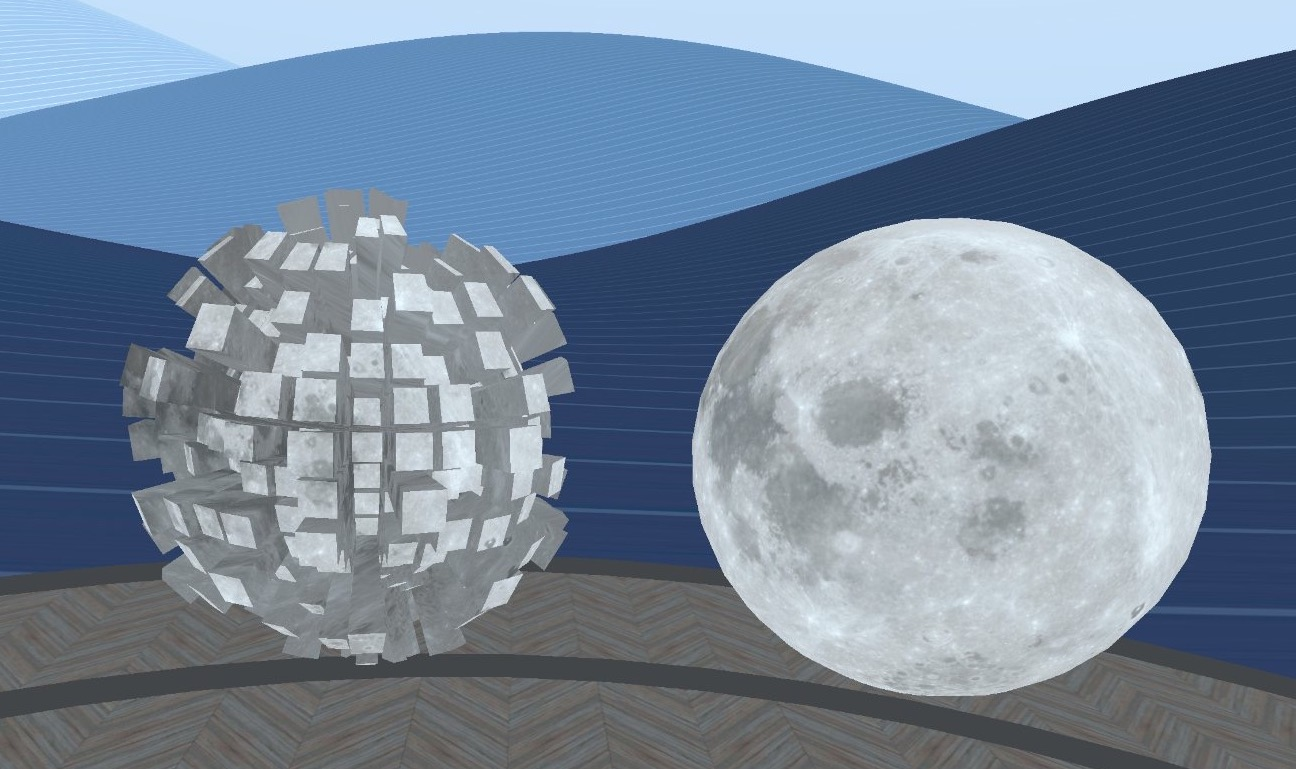
\includegraphics[keepaspectratio, width=0.7\linewidth]{figures/geometry-shader.jpg}
  \caption{
    図右の月のオブジェクトに対して,Geometry Shaderを適応し,
    球体内部のポリゴンの追加と,頂点の編集を行い,図左のオブジェクトをレンダリングする様子.
  }
  \label{fig:geometry-shader}
\end{figure}

\subsection{カラーマップ以外のテクスチャの利用}

テクスチャマッピングは,メッシュ表面のベースカラーを表現する以外にも多くの利用方法がある.
バンプマップ\cite{bump-mapping}ではテクスチャにメッシュの表面からの高さの変位を
エンコーディングし,面の法線ベクトルの微妙な変化を計算して,シェーディングに利用することで
細やかな表面の表現が可能になる.
また,テクスチャにメッシュ表面の法線ベクトルをエンコーディングした法線マップを用いた
レンダリング手法\cite{normal-map}や,
テクスチャにメッシュ表面の光沢の度合いをエンコーディングするスペキュラマップなどは
一般によく用いられる.

本システムではテクスチャの利用の仕方も特定の方法に限定しないため,これらのようなテクスチャの
利用方法も実現できる.
ここでは本レンダリングシステムでバンプマップを用ることで,月面の細やかな法線の揺らぎを
計算し,月面の凹凸による陰を表現できることを確認した.

\begin{figure}[htbp]
  \begin{minipage}[t]{\linewidth}
    \centering
    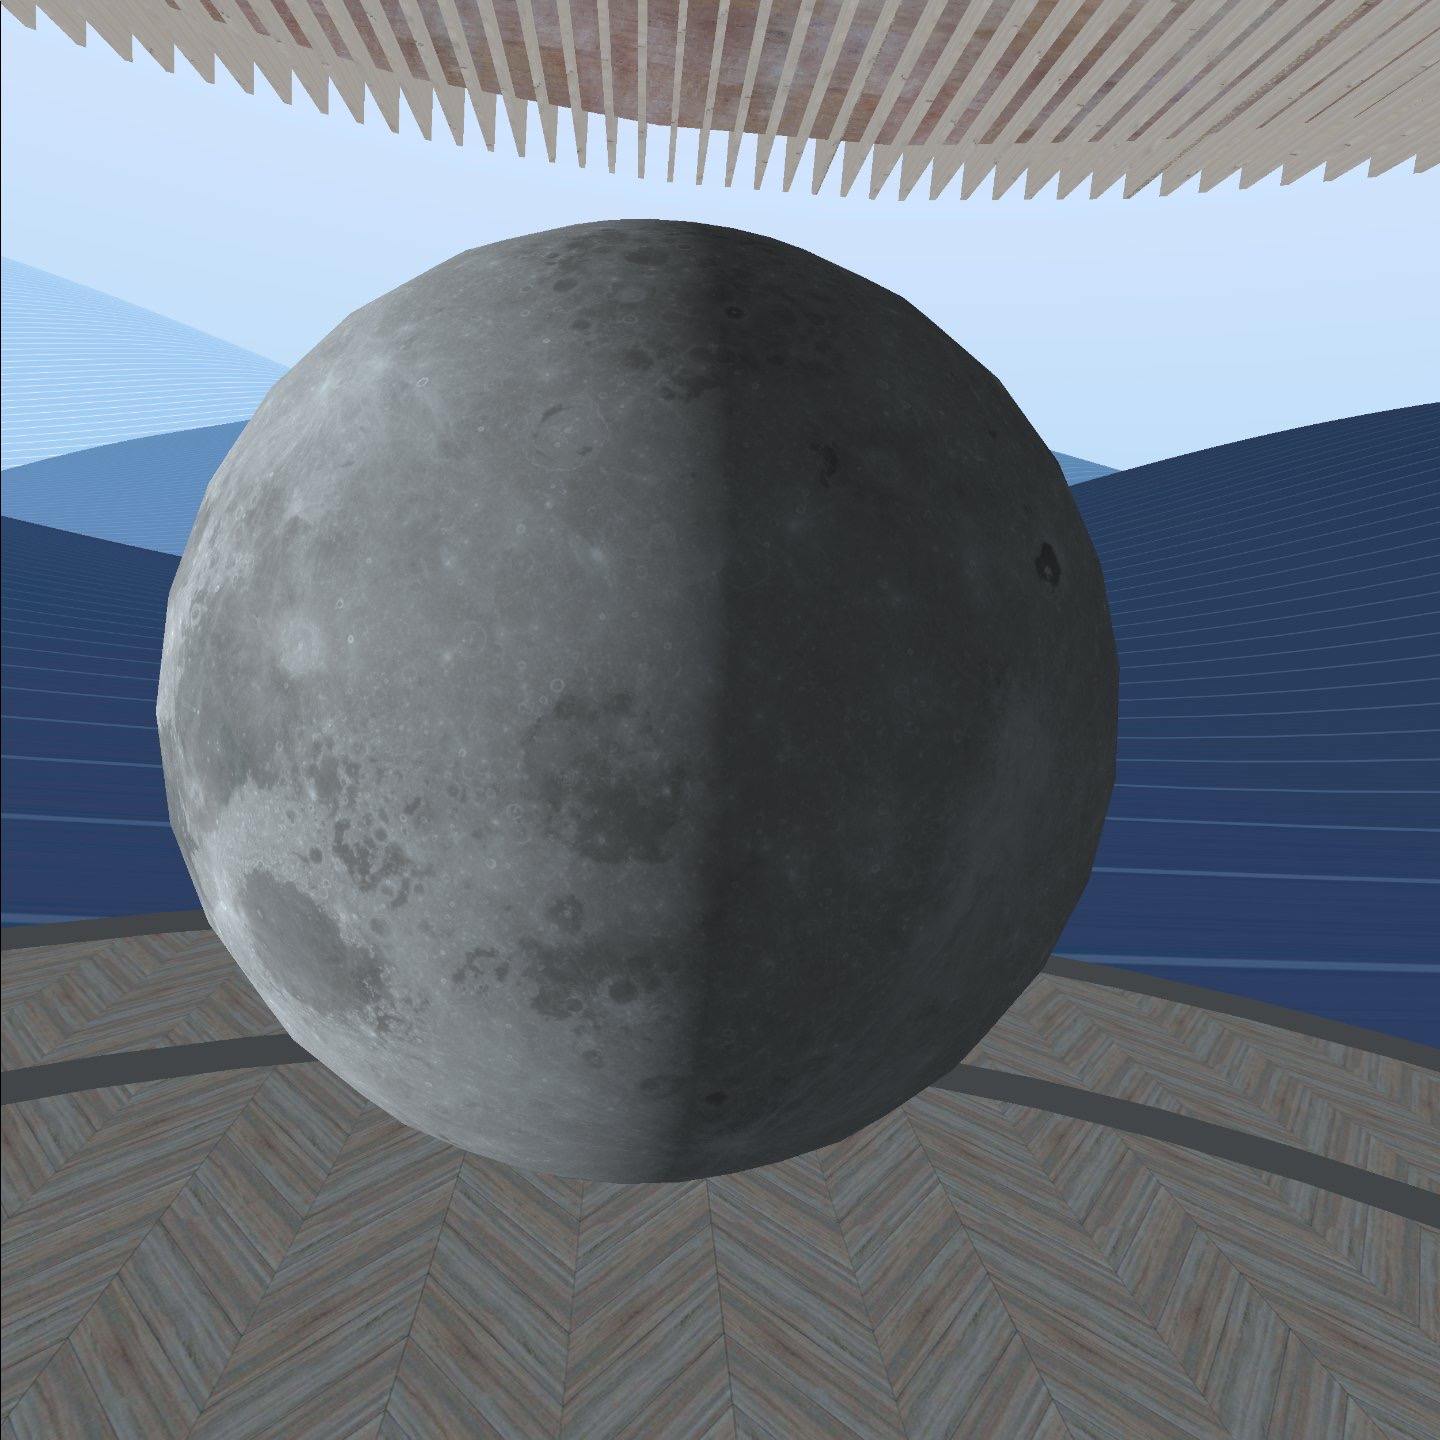
\includegraphics[keepaspectratio, width=0.49\linewidth]{figures/no-bump-map.jpg}
  \end{minipage}
  \begin{minipage}[t]{0.49\linewidth}
    \captionsetup[sub]{margin=0.1cm}
    \centering
    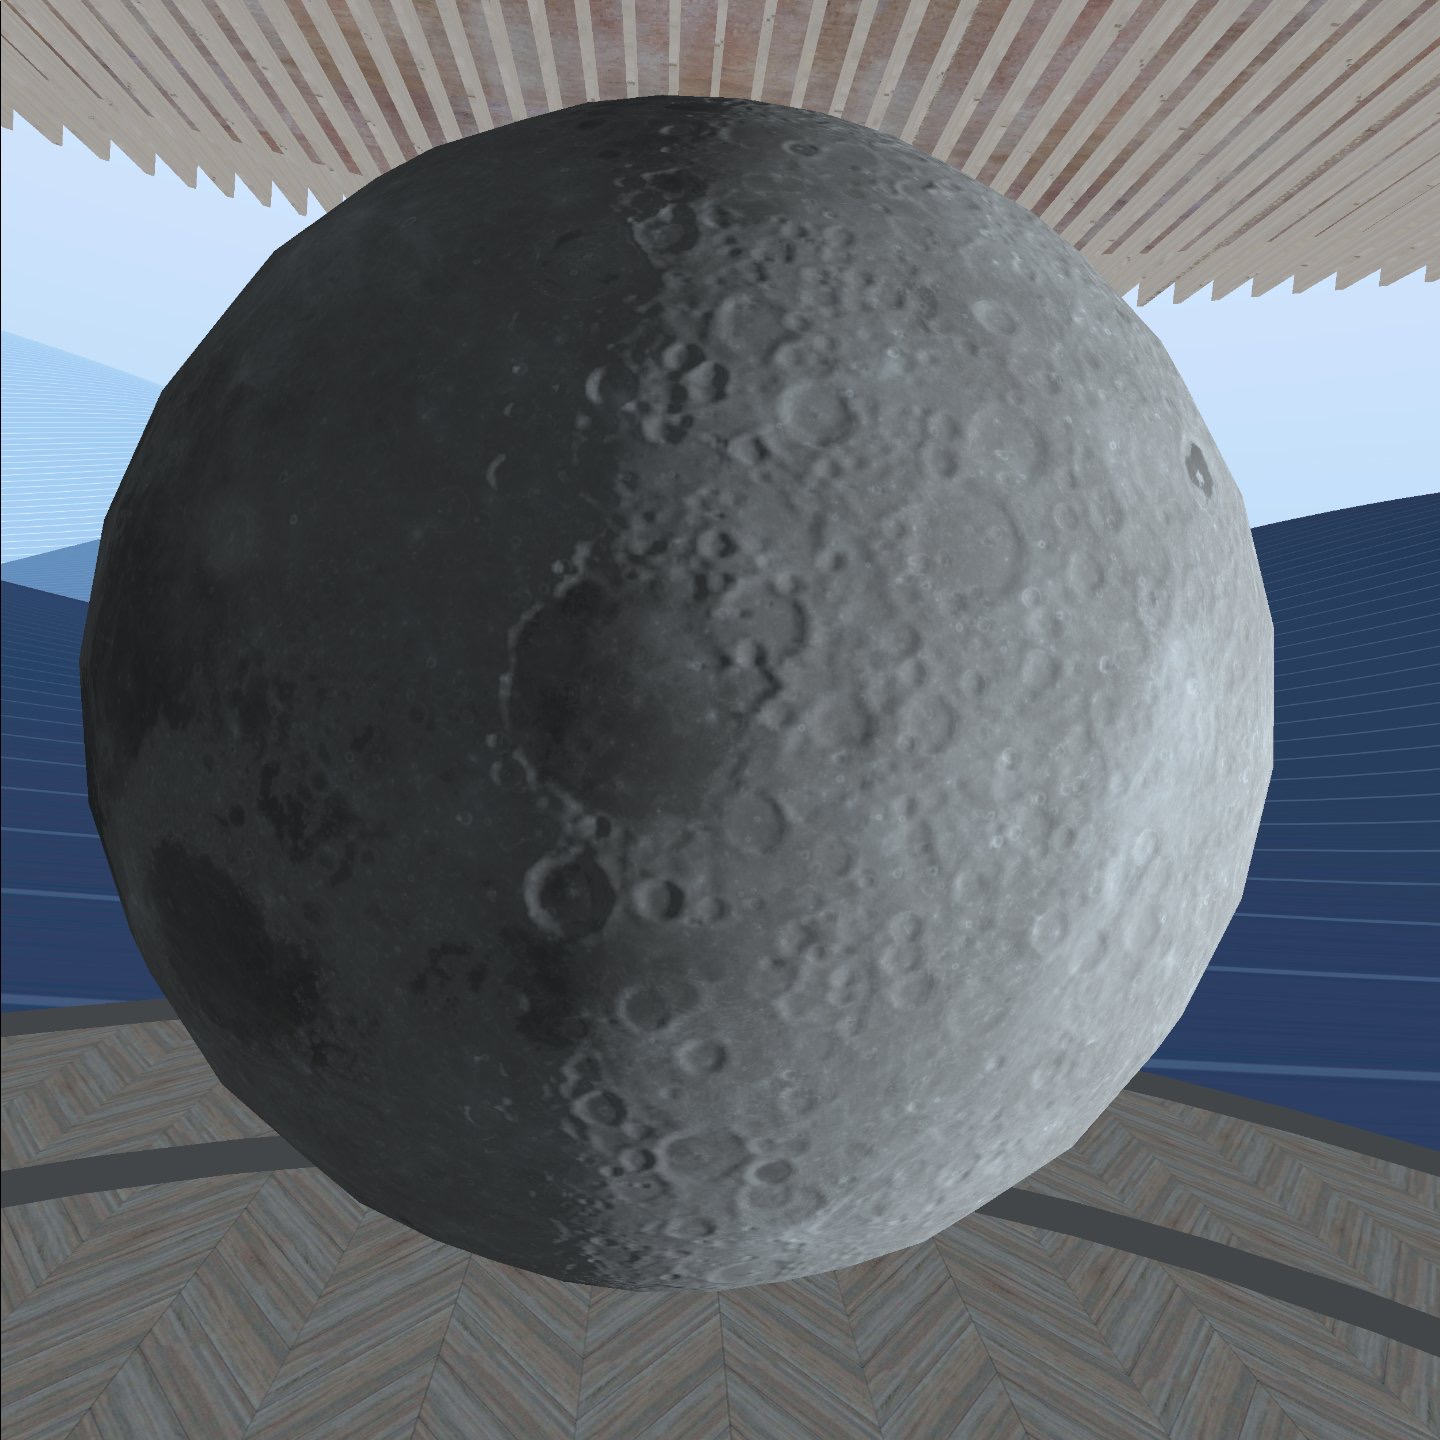
\includegraphics[keepaspectratio, width=\linewidth]{figures/bump-map0.jpg}
  \end{minipage}
  \begin{minipage}[t]{0.49\linewidth}
    \captionsetup[sub]{margin=0.1cm}
    \centering
    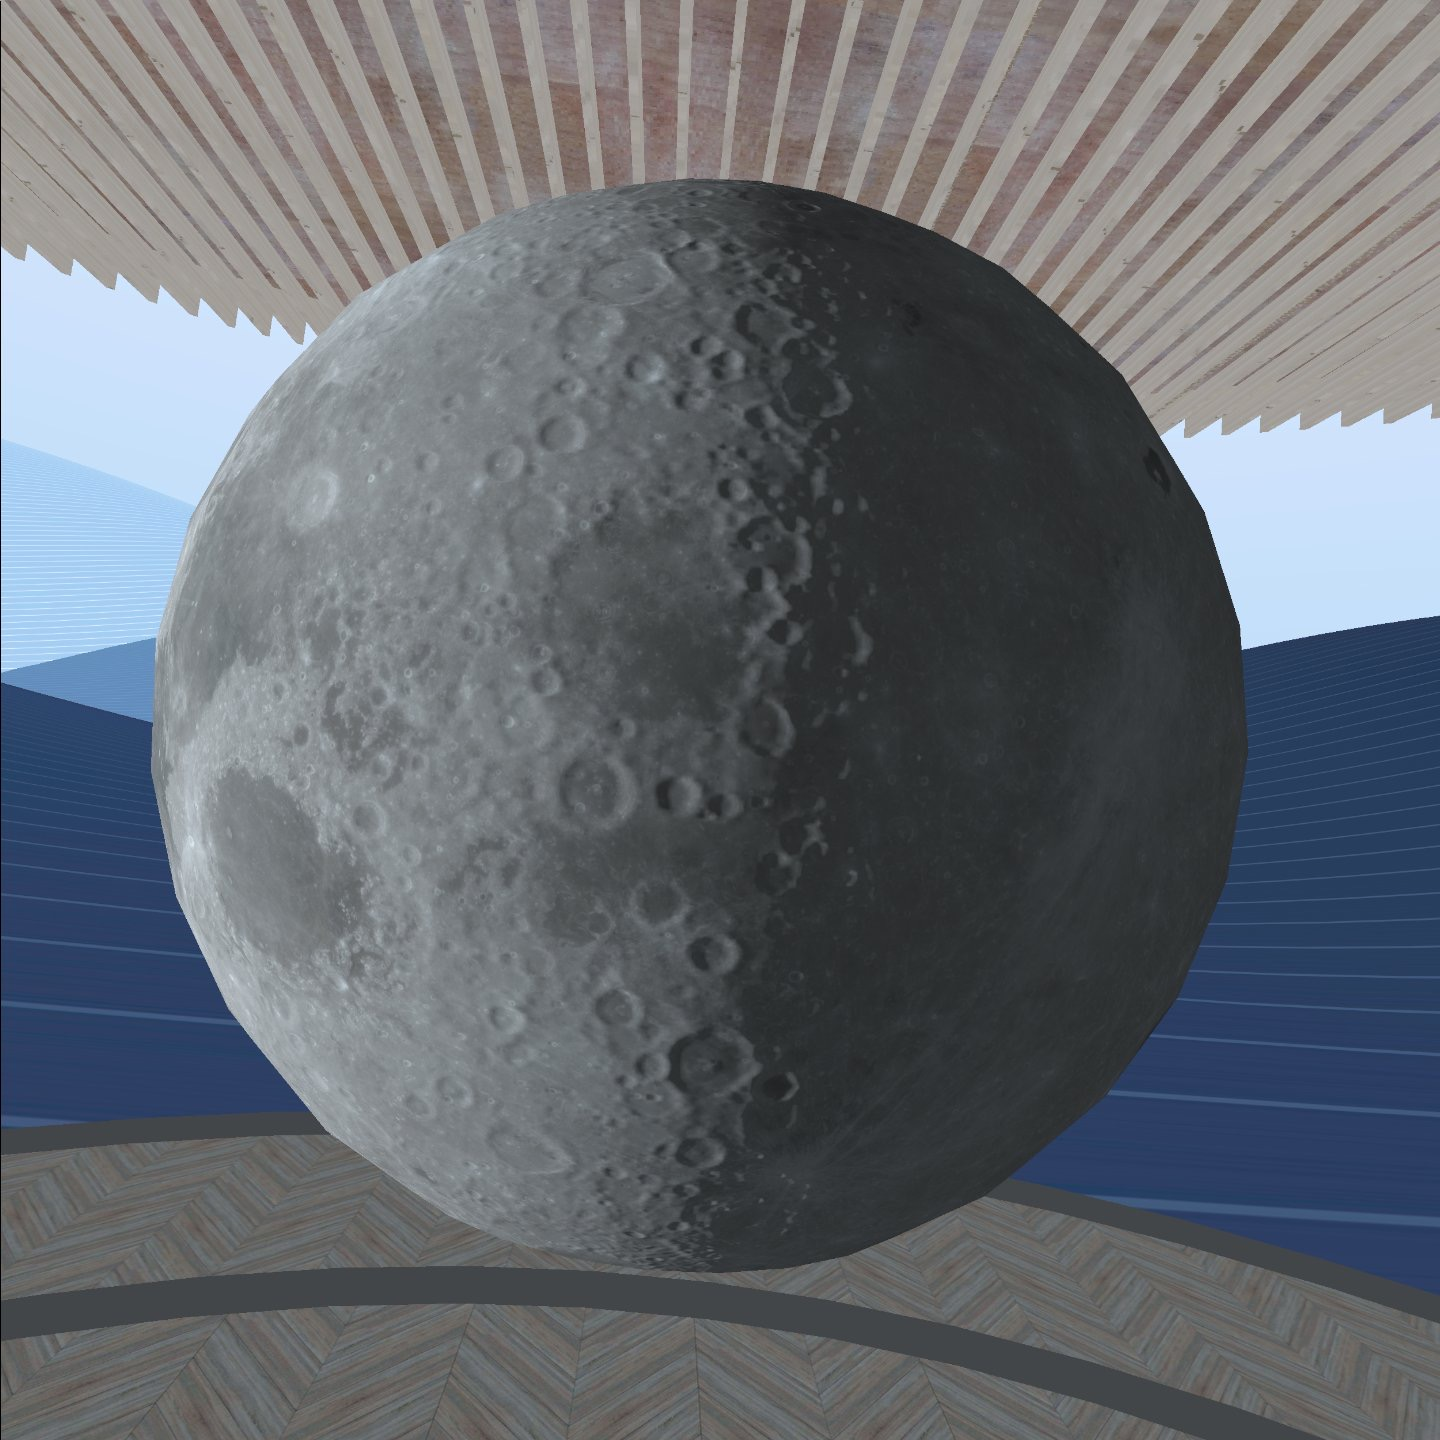
\includegraphics[keepaspectratio, width=\linewidth]{figures/bump-map1.jpg}
  \end{minipage}
  \caption{
    本レンダリングシステムでバンプマップを適用し,月面の凹凸をレンダリングに反映させた様子.
    図上はバンプマップを適用しない場合.
    図下の左右はバンプマップを適用し,光源の位置を変化させた様子.
  }
  \label{fig:bumpmap}
\end{figure}


% Sphere Tracing はRay Marching手法の1つで,

% 実験内容
% * レンダリング性能
% * 自由度
% Limitation
% * マルチパスレンダリング
% * 他のApplicationの影
% * シングルパスステレオレンダリング

\section{まとめ}

% \subsection{まとめ}

% \subsection{限界}

% \subsection{今後の課題}

% * 今後の展開
% ** PBR ベースなど
